\documentclass[12pt,a4paper]{article}
\usepackage[utf8]{inputenc}
\usepackage{geometry}
\usepackage{graphicx}
\usepackage{amsmath}
\usepackage{hyperref}
\usepackage{lipsum}
\usepackage{longtable}
\usepackage{booktabs}


% Page layout
\geometry{top=1in, bottom=1in, left=1in, right=1in}

% Title settings
\begin{document}
\begin{titlepage}
    \centering
    \vspace*{1cm}

    % Menambahkan logo atau gambar yang diinginkan di tengah
   

    {\LARGE \textbf{Deep Learning Course}}\\[0.5cm]
    {\Large \textbf{Final Project Report}}\\[1.5cm]

     
\includegraphics[width=0.5\textwidth]{Image/Logo-Resmi-Unhas-1.png}\\[1cm] % Ganti dengan nama file gambar Anda
    
    % Daftar penulis
    \textbf{Disusun oleh:}\\[0.5cm]
    \begin{tabbing}
        \hspace{3cm} \= NURUL ALYA \hspace{3cm} \= H071221009 \kill
        \> NURUL ALYA \hspace{5.27cm} \= H071221009 \\
        \> REZQIA NURQALBI \hspace{4cm} \= H071221025 \\
        \> ANDI MUTHIA MULIA PUTRI \hspace{2cm} \= H071221041 \\
    \end{tabbing}
    
    \vfill
    
    % Informasi universitas dan tanggal
    \textbf{Universitas Hasanuddin}\\
    \textbf{Makassar, Indonesia}\\[0.5cm]
    \textbf{\today}
    
\end{titlepage}


\tableofcontents
\newpage

% 1. Introduction
\section{\uppercase Introduction}
\begin{itemize}
    \item \textbf {Background and context of the project}

   \hspace{0.5cm} Teknologi pengenalan gestur tangan telah berkembang pesat, terutama dengan dukungan machine learning dan deep learning yang semakin canggih. Salah satu aplikasi yang banyak dikembangkan adalah pengenalan gestur hand digit (angka 1 hingga 5), yang memiliki potensi besar untuk meningkatkan interaksi manusia-komputer (Human-Computer Interaction atau HCI). Teknologi ini dapat digunakan untuk berbagai kebutuhan, seperti komunikasi sederhana, kontrol perangkat berbasis IoT, hingga interaksi dengan robot asisten.
   
   \hspace{0.5cm} Namun, pengembangan teknologi ini menghadapi tantangan besar, terutama dalam hal penyediaan dataset yang cukup bervariasi untuk melatih model deep learning. Variasi dataset diperlukan agar model dapat mengenali gestur tangan dengan akurasi tinggi dalam berbagai kondisi lingkungan, termasuk jarak, pencahayaan, dan latar belakang. Dengan menciptakan dataset yang beragam, teknologi pengenalan gestur tangan dapat diterapkan dalam situasi nyata dan mendukung pengembangan aplikasi berbasis kecerdasan buatan yang lebih andal.

    \item \textbf {Problem statement}
    
    \begin{itemize}
        \item \textbf{Kurangnya Dataset Berkualitas:} Teknologi pengenalan gestur tangan, khususnya untuk hand digit 1 hingga 5, sering terhambat oleh kurangnya dataset yang mencakup berbagai kondisi lingkungan.

        \item \textbf{Pengaruh Faktor Lingkungan:} Variasi jarak, pencahayaan, dan latar belakang yang berbeda dapat memengaruhi akurasi model deep learning dalam mengenali gestur tangan.

        \item \textbf{Keterbatasan Implementasi Luas:} Kendala ini menghambat pengaplikasian teknologi pengenalan gestur tangan secara luas, terutama pada sistem yang membutuhkan keandalan tinggi, seperti robot asisten atau perangkat IoT.
        
    \end{itemize}

    \item \textbf {Objectives of the research}


    \begin{itemize}
    \item \textbf{Menyediakan Dataset yang Bervariasi:}  
    Mengembangkan dataset pengenalan hand digit 1 hingga 5 yang mencakup variasi jarak, pencahayaan, dan latar belakang. Dataset ini dirancang agar model deep learning dapat dilatih untuk mengenali gestur tangan secara andal di berbagai kondisi lingkungan.
    
    \item \textbf{Meningkatkan Akurasi Model Deep Learning:}  
    Menggunakan dataset baru untuk meningkatkan akurasi model deep learning, seperti Convolutional Neural Networks (CNN), dalam mengenali gestur tangan.
    
    \item \textbf{Mendukung Pengembangan Aplikasi Berbasis AI}  
    Memfasilitasi pengembangan teknologi berbasis pengenalan gestur tangan untuk aplikasi interaksi manusia-komputer, perangkat IoT, dan robot asisten, khususnya dalam sektor layanan, seperti pemesanan ruangan karaoke.
    
    \item \textbf{Mendorong Implementasi Teknologi Berbasis Gestur:}  
    Membantu mengintegrasikan teknologi pengenalan gestur tangan dalam aplikasi sehari-hari, sehingga proses menjadi lebih cepat, intuitif, dan bebas sentuhan.
    \end{itemize}

\hspace{0.5cm} Dengan tercapainya tujuan-tujuan ini, pengembangan teknologi pengenalan gestur tangan diharapkan dapat memberikan manfaat yang signifikan bagi berbagai bidang, dari hiburan hingga interaksi berbasis AI yang lebih luas.

\end{itemize}

% 2. Related Works
\section{\uppercase Related Works}
\begin{itemize}
    \item \textbf {Literature review of relevant papers and articles}
    
    \hspace{0.5cm}Penelitian seperti yang dilakukan oleh Domahs et al. (2010, dalam Cognition) menunjukkan bahwa kebiasaan menghitung menggunakan jari memengaruhi cara angka diproses, dan mendukung asumsi bahwa efek ini dimodulasi oleh budaya. Namun, tingkat keberagaman budaya dalam kebiasaan menghitung dengan jari secara umum sangat diremehkan di bidang penelitian, yang pada gilirannya membatasi pertanyaan dan desain penelitian.
    
    \hspace{0.5cm}Dalam hal ini, Bender dan Beller (2012) mengeksplorasi diversitas budaya dalam penggunaan jari untuk menghitung angka. Mereka menemukan bahwa sistem penghitung jari bervariasi dalam aspek seperti jari yang digunakan untuk memulai, tangan yang digunakan, dan orientasi gerakan (misalnya, dari tangan tertutup ke terbuka atau sebaliknya). Studi ini menegaskan bahwa gestur jari tidak hanya merupakan alat kognitif alami, tetapi juga sangat dipengaruhi oleh kode budaya tertentu, yang mencerminkan kompleksitas interaksi antara faktor biologis dan sosial dalam representasi angka.
    
    \hspace{0.5cm}Penerapan konsep ini menjadi relevan dalam pengembangan teknologi pengenalan gestur jari, terutama untuk mengenali angka yang ditunjukkan dengan tangan. Teknologi ini merupakan bagian penting dari interaksi manusia-komputer (Human-Computer Interaction atau HCI) dan digunakan dalam berbagai aplikasi, seperti komunikasi non-verbal, kontrol perangkat berbasis IoT, hingga interaksi dengan robot asisten. Sistem ini memanfaatkan teknologi berbasis visi, sensor radar, dan algoritma pembelajaran mesin untuk memahami dan menganalisis gestur tangan.
    
    \hspace{0.5cm}Namun, salah satu tantangan utama dalam pengembangan teknologi ini adalah menyediakan dataset yang mencakup variasi kondisi lingkungan, seperti pencahayaan, jarak, dan latar belakang yang berbeda. Variasi ini diperlukan untuk melatih model agar mampu mengenali gestur tangan dengan akurasi tinggi dalam berbagai skenario nyata. Dengan mengatasi tantangan ini, pengenalan gestur jari dapat menjadi lebih andal dan dapat diterapkan secara luas dalam berbagai sistem berbasis AI.

    \item \textbf {Comparison of different approaches and their results}
    \begin{itemize}
        \item \textbf{Nature and Culture or Finger Counting: Diversity and Representational Effects of An Embodied Cognitive Tool}
        
        \hspace{0.5cm} Penelitian ini menggunakan pendekatan studi etnografis dan kognitif tentang variasi budaya dalam penghitungan jari yang hasilnya menunjukkan variasi budaya dalam penghitungan jari yang memengaruhi representasi dan pemrosesan angka serta pendekatan pendidikan. Relevansi dan implikasinya menyoroti pentingnya konteks budaya dalam memahami dan mengaplikasikan gestur tangan, relevan untuk desain dataset yang mempertimbangkan variasi budaya.

        \item \textbf{Implementing a Hand Gesture Recognition System Based on Range-Doppler Map}
        
        \hspace{0.5cm} Penelitian ini menggunakan pendekatan penggunaan sinyal radar berbasis peta Range-Doppler untuk mengenali gestur tangan yang hasilnya mencapai akurasi 98\% dalam klasifikasi gestur, dengan fleksibilitas tinggi untuk berbagai skenario penggunaan. Relevansi dan implikasinya menekankan efisiensi pendekatan berbasis radar, namun tantangan pada gestur mikro dan lingkungan beragam tetap relevan untuk dibandingkan dengan metode visual.

        \item \textbf{Hybrid CNN-SVM Classifier for Handwritten Digit Recognition}
        
        \hspace{0.5cm} Penelitian ini menggunakan kombinasi CNN dan SVM untuk mengenali angka tulisan tangan pada dataset MNIST yang hasilnya akurasi tinggi sebesar 99,28\% menunjukkan efektivitas pendekatan hibrida dalam mengenali pola kompleks. Relevansi dan implikasinya menggarisbawahi pentingnya kerangka kerja yang canggih dalam mencapai akurasi tinggi, relevan dengan penelitian pengenalan gestur tangan berbasis visual.

    \end{itemize}
    
    \item \textbf {Justification for your chosen methodology}
    
    \hspace{0.5cm}Metodologi yang dipilih untuk proyek ini didasarkan pada kebutuhan untuk mengatasi keterbatasan yang diidentifikasi dalam penelitian sebelumnya terkait keberagaman dataset dan representasi budaya dalam pengenalan gestur. Dengan fokus pada dataset yang menangkap berbagai gestur digit tangan dalam kondisi yang bervariasi, proyek ini bertujuan untuk:

    \begin{itemize}
    \item \textbf{Meningkatkan Ketahanan Model: } Dengan menyertakan contoh beragam dari digit tangan dari berbagai sudut pandang, jarak, dan kondisi pencahayaan, dataset akan memungkinkan model untuk lebih baik menggeneralisasi di berbagai skenario dunia nyata.

    \item \textbf{Mendukung Adaptabilitas Budaya: }  Mengingat kebiasaan menghitung dengan jari berbeda secara budaya, dataset akan mencakup variasi dalam representasi gestur untuk memenuhi audiens global.

    \item \textbf{Memanfaatkan Teknik Lanjutan: }  Menggunakan CNN dan arsitektur deep learning lainnya akan memastikan bahwa sistem mampu mencapai akurasi tinggi dalam mengenali gestur digit tangan, sehingga meningkatkan interaksi manusia-komputer.
    
    \end{itemize} 

\end{itemize}

% 3. Dataset and Material
\section{\uppercase Dataset and Material}
\begin{itemize}
    \item  \textbf {Source of the dataset}
    
    \hspace{0.5cm} Dataset yang digunakan dalam proyek ini adalah Natural Hand Digit Dataset yang dikembangkan secara mandiri. Dataset ini dirancang untuk mendukung pengenalan gestur tangan berupa angka 1 hingga 5, yang relevan untuk aplikasi berbasis Human-Computer Interaction (HCI) dan IoT.

    Metode Pengambilan Data:

    \begin{itemize}
    \item \textbf{Kamera:} Pengambilan data dilakukan menggunakan smartphone dengan spesifikasi berikut:
    \begin{itemize}
        \item Resolusi video Ultra HD 4K (3840 x 2160p) pada 30 fps.
        \item Sistem Operasi: Android 14 dengan chipset Exynos 1480.
    \end{itemize}
    
    \item \textbf{Variasi Data:} Data dikumpulkan dengan variasi pengambilan berikut:
    \begin{itemize}
        \item Tiga jarak pengambilan: 50 cm, 1 m, dan 2 meter.
        \item Kondisi pencahayaan rendah untuk meniru situasi dunia nyata.
        \item Background netral (putih) agar fokus hanya pada gestur tangan.
    \end{itemize}

    \item \textbf{Tinggi pengambilan data:} Kamera dipasang pada ketinggian 125 cm menggunakan tripod untuk mencerminkan tinggi rata-rata bahu manusia, menghasilkan perspektif yang konsisten untuk setiap pengambilan data.

    \item \textbf{Skenario Pengambilan Data:} Pengambilan data dilakukan dengan merekam video angka 1 hingga 5 menggunakan berbagai posisi tangan dari beberapa individu. Hal ini untuk memastikan keberagaman dalam representasi gestur tangan yang dapat digunakan oleh model dalam berbagai situasi.

    \item \textbf{Jumlah Data yang dikumpulkan per pekan :}

    \renewcommand{\arraystretch}{1.5} % Menambah jarak antar baris

\subsection*{Pekan 11 dan Pekan 12}

\begin{tabular}{|c|c|c|c|}
\hline
\textbf{Digit} & \textbf{Jarak} & \textbf{Pekan 11 (Jumlah Data)} & \textbf{Pekan 12 (Jumlah Data)} \\ \hline
1 & 50cm & 90 data & 30 data \\ \hline
2 & 50cm & 90 data & 30 data \\ \hline
3 & 50cm & 90 data & 30 data \\ \hline
4 & 50cm & 90 data & 30 data \\ \hline
5 & 50cm & 90 data & 30 data \\ \hline
1 & 1m & 90 data & 30 data \\ \hline
2 & 1m & 90 data & 30 data \\ \hline
3 & 1m & 90 data & 30 data \\ \hline
4 & 1m & 90 data & 30 data \\ \hline
5 & 1m & 90 data & 30 data \\ \hline
1 & 2m & 90 data & 30 data \\ \hline
2 & 2m & 90 data & 30 data \\ \hline
3 & 2m & 90 data & 30 data \\ \hline
4 & 2m & 90 data & 30 data \\ \hline
5 & 2m & 90 data & 30 data \\ \hline
\multicolumn{2}{|c|}{\textbf{Total Data}} & \textbf{1350 data} & \textbf{900 data} \\ \hline
\end{tabular}

\renewcommand{\arraystretch}{1.5} % Menambah jarak antar baris

\subsection*{Pekan 13 dan Pekan 14}

\begin{tabular}{|c|c|c|c|}
\hline
\textbf{Digit} & \textbf{Jarak} & \textbf{Pekan 13 (Jumlah Data)} & \textbf{Pekan 14 (Jumlah Data)} \\ \hline
1 & 50cm & 90 data & 90 data \\ \hline
2 & 50cm & 90 data & 90 data \\ \hline
3 & 50cm & 90 data & 90 data \\ \hline
4 & 50cm & 90 data & 90 data \\ \hline
5 & 50cm & 90 data & 90 data \\ \hline
1 & 1m & 90 data & 90 data \\ \hline
2 & 1m & 90 data & 90 data \\ \hline
3 & 1m & 90 data & 90 data \\ \hline
4 & 1m & 90 data & 90 data \\ \hline
5 & 1m & 90 data & 90 data \\ \hline
1 & 2m & 90 data & 90 data \\ \hline
2 & 2m & 90 data & 90 data \\ \hline
3 & 2m & 90 data & 90 data \\ \hline
4 & 2m & 90 data & 90 data \\ \hline
5 & 2m & 90 data & 90 data \\ \hline
\multicolumn{2}{|c|}{\textbf{Total Data}} & \textbf{1350 data} & \textbf{1350 data} \\ \hline
\end{tabular}
    
\end{itemize}

    \item  \textbf {Preprocessing steps.}
    
    Proses preprocessing dataset meliputi:

    \begin{itemize}
    \item \textbf{Pembagian Data:} 
    \begin{itemize}
        \item Dataset dibagi menjadi dua subset: training (80\%) dan testing (20\%) menggunakan fungsi Python untuk memastikan distribusi yang seimbang.
        \item File dipindahkan secara terstruktur berdasarkan kelas.
    \end{itemize}

    \item \textbf{Resize dan Normalisasi:} 
    \begin{itemize}
        \item Semua gambar diubah ukurannya menjadi 224x224 piksel.
        \item Nilai piksel dinormalisasi ke skala [0, 1] menggunakan \texttt {ImageDataGenerator}.
    \end{itemize}

    \item \textbf{Augmentasi Data:} 
    \begin{itemize}
        \item Augmentasi gambar diterapkan menggunakan \texttt {ImageDataGenerator} untuk menambah variasi dataset, seperti flipping, rotasi, dan zoom.
    \end{itemize}

    \item \textbf{Pemeriksaan Data:}

    \begin{itemize}
        \item Dataset dianalisis untuk memeriksa distribusi kelas menggunakan plot distribusi data.
        \item Contoh gambar dari setiap kelas ditampilkan untuk memverifikasi kualitas dan label.
    \end{itemize}

\end{itemize}

    \item  \textbf{Features and labels included in the data.}
    \begin{itemize}
    \item \textbf{Fitur (Features):} 
    Gambar tangan yang menampilkan gestur angka direpresentasikan sebagai matriks nilai piksel berukuran 224x224x3 (RGB). Setiap gambar adalah representasi visual dari angka yang ditunjukkan dengan tangan dalam bentuk gestur.
    
    \item \textbf{Label (Output):} 
    Kategori angka yang ditunjukkan oleh gestur tangan pada gambar, yaitu angka 1, 2, 3, 4, atau 5. Label ini digunakan sebagai target yang diprediksi oleh model dalam proses pelatihan.
\end{itemize}

\begin{figure}[h]
    \centering
    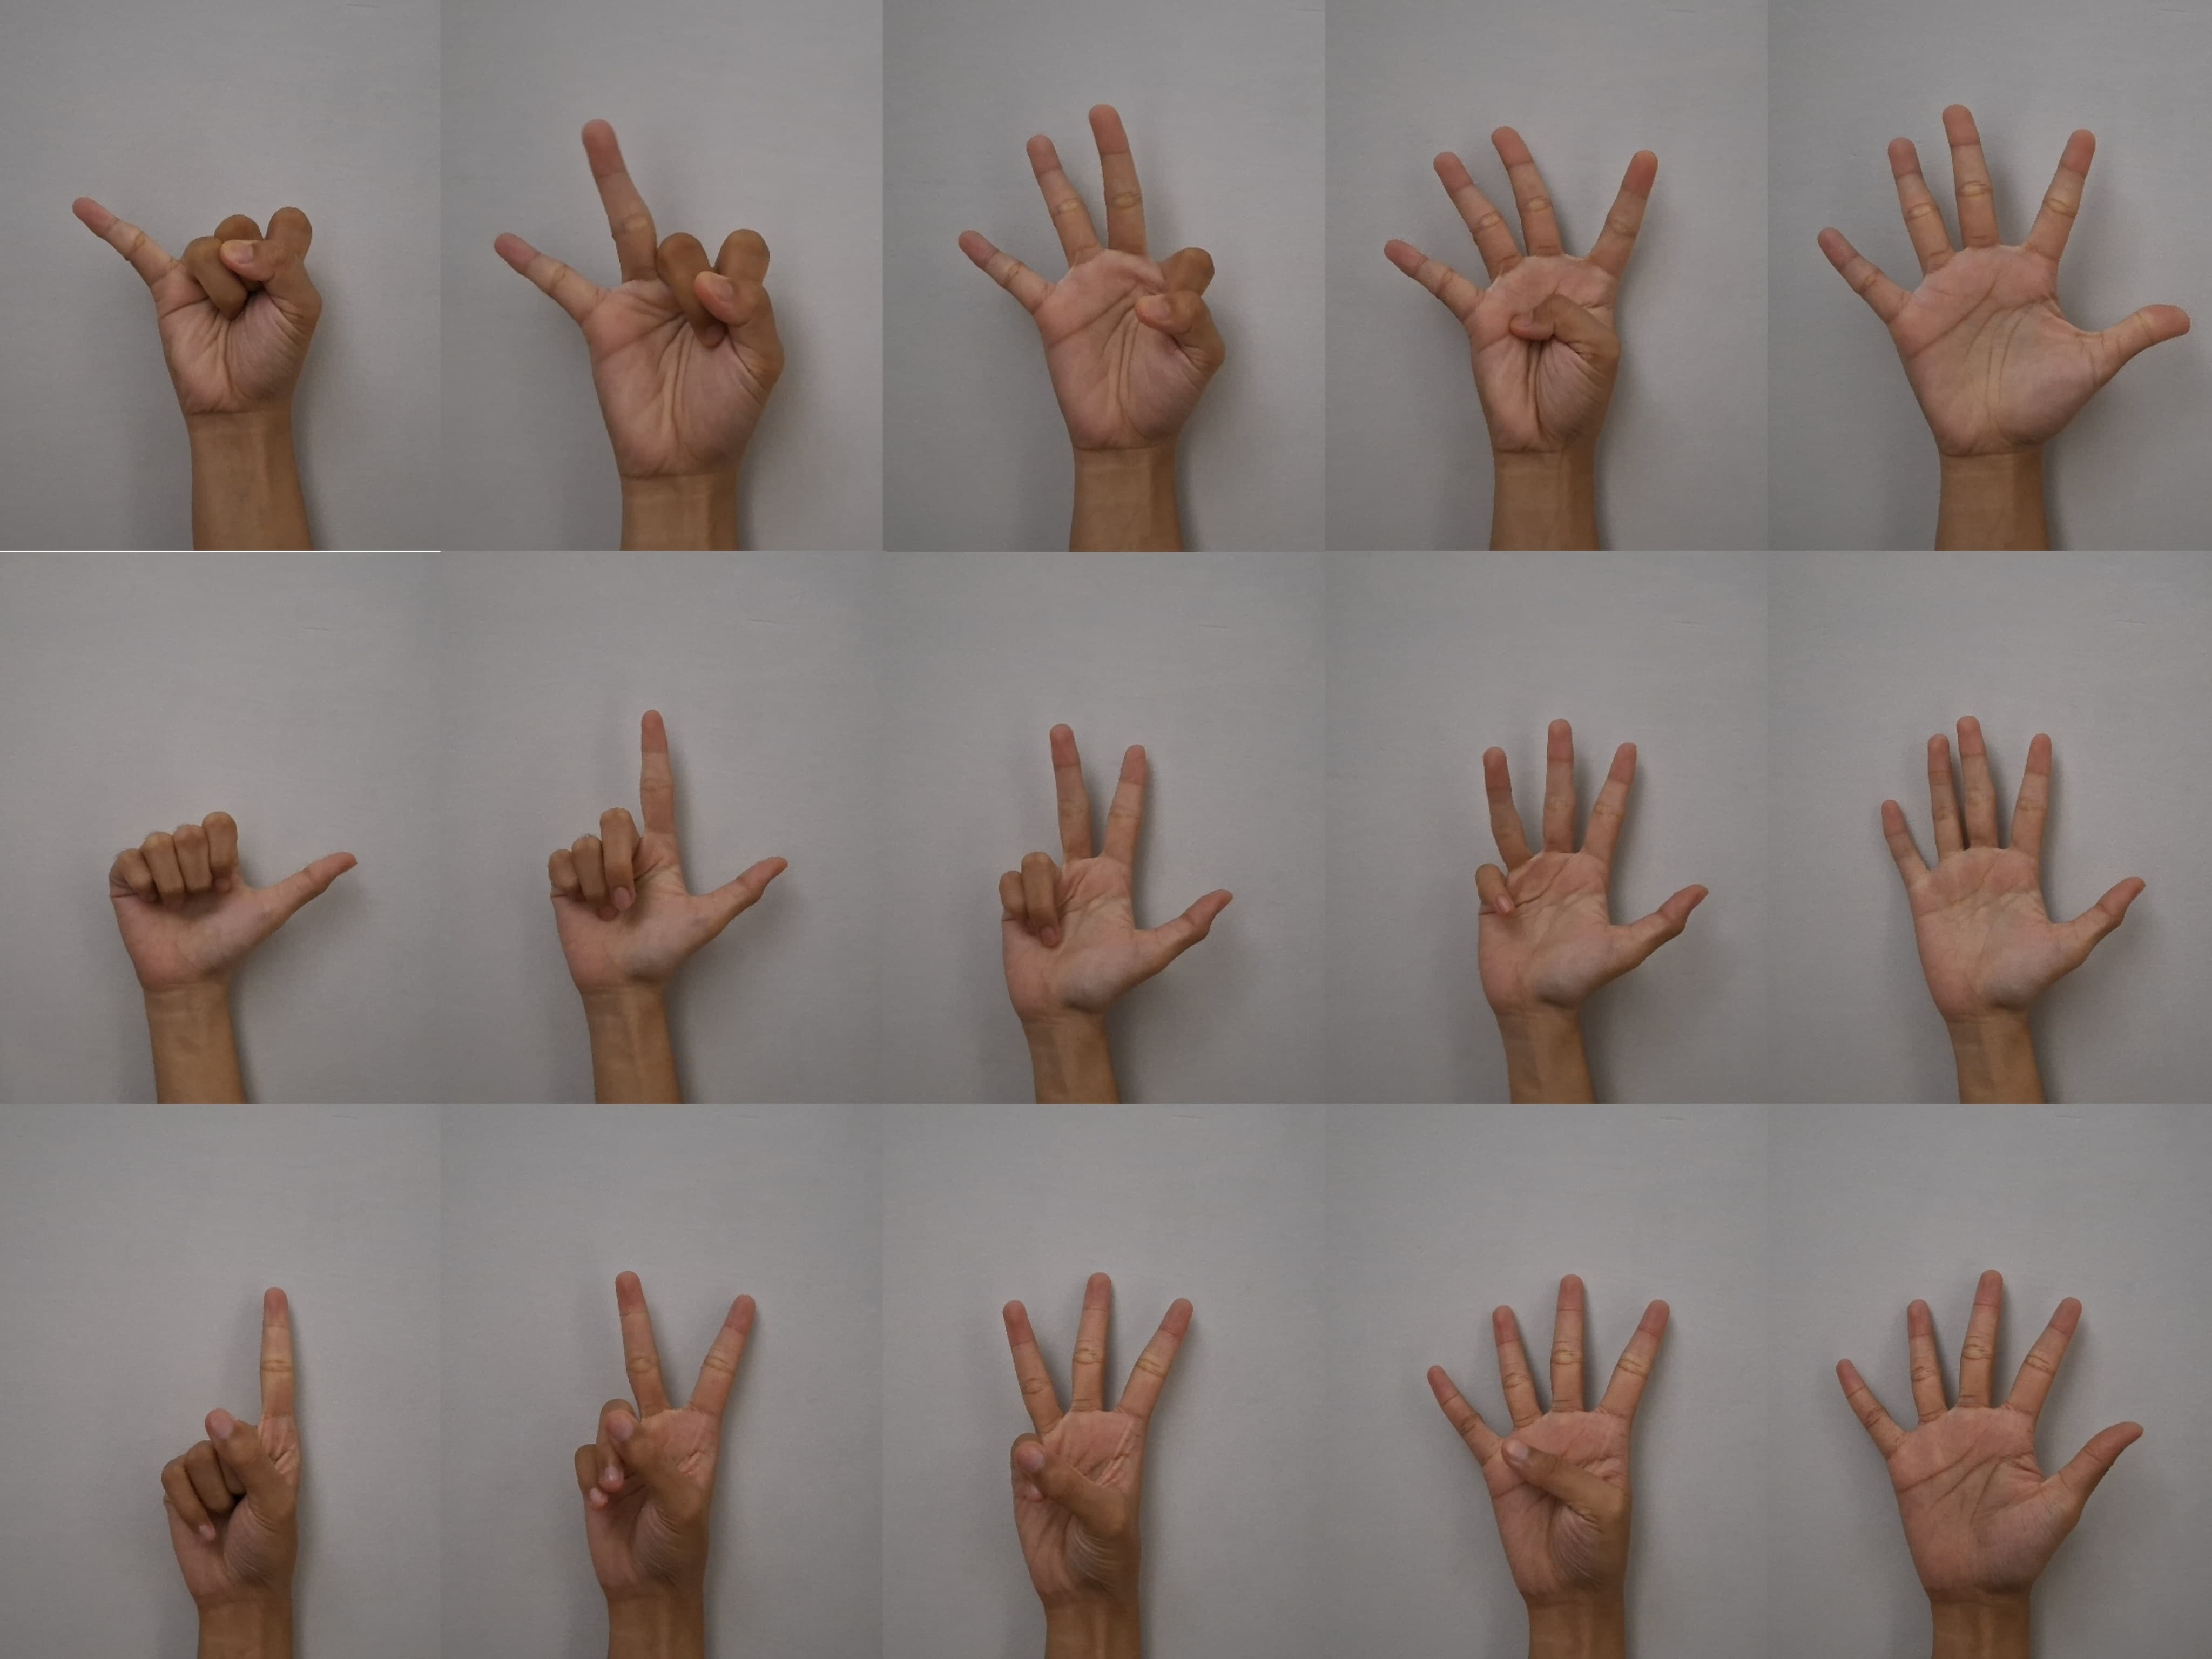
\includegraphics[width=0.6\textwidth]{Image/Contoh Tangan.jpeg}
    \caption{Contoh gambar dari masing-masing kategori angka}
    \label{fig:hand_gesture_example}
\end{figure}


 \item \textbf{Tools, Libraries, and Frameworks}
 
Beberapa alat dan pustaka yang digunakan dalam proyek ini adalah sebagai berikut:

\begin{itemize}
    \item \textbf{Tools:} Google Colab
\end{itemize}
\begin{figure}[h]
    \centering
    
\includegraphics[width=0.3\textwidth]{Image/colabPng.png}
    \caption{Logo Google Colab}
    \label{fig:Logo_google_colab}
\end{figure}
\hspace{0.5cm} Google Colab digunakan sebagai platform berbasis cloud untuk menulis, menjalankan, dan mempercepat kode dengan dukungan GPU/TPU gratis.


\begin{itemize}
    \item \textbf{Bahasa Pemrograman:} Python
\end{itemize}
\begin{figure}[h]
    \centering
    
\includegraphics[width=0.2\textwidth]{Image/pythonpng.png}
    \caption{Logo Bahasa Pemrograman Python}
    \label{fig:Logo_python}
\end{figure}
\hspace{0.5cm} Python digunakan untuk mengembangkan kode yang mencakup pengolahan data, pemrosesan gambar, pembangunan model deep learning, evaluasi performa, dan visualisasi hasil.

\begin{itemize}
    \item \textbf{Library untuk Preprocessing dan Visualisasi:}
    \begin{figure}[h]
    \centering
    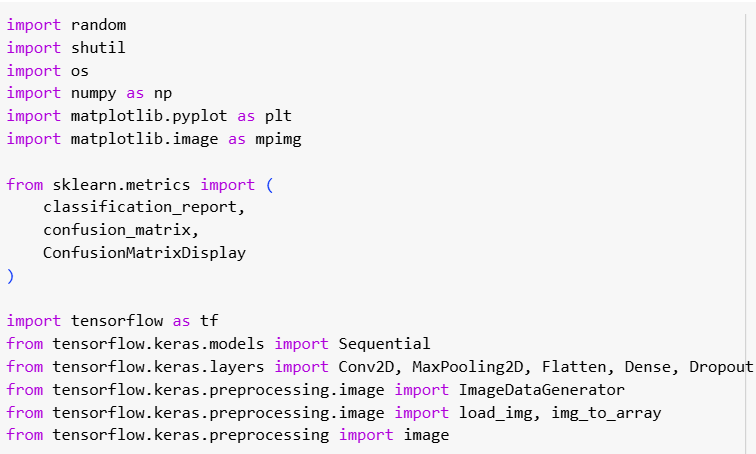
\includegraphics[width=0.6\textwidth]{Image/Import.png}
    \caption{Library Yang Digunakan}
    \label{fig:Library}
\end{figure}
\begin{itemize}
    \item \textbf{Manipulasi File dan Folder:} 
    Pustaka seperti \texttt{os}, \texttt{shutil}, dan \texttt{random} digunakan untuk mengelola file dan folder, seperti memindahkan, menyalin, atau mengacak file dalam direktori. Hal ini berguna saat menyiapkan dataset atau mengatur struktur folder.

    \item \textbf{Pengolahan Data dan Visualisasi:} 
    \texttt{numpy} digunakan untuk operasi matematika dan manipulasi array yang efisien, sementara \texttt{matplotlib} membantu memvisualisasikan data, seperti menampilkan gambar, grafik akurasi, atau matriks kebingungan hasil evaluasi.

   \item \textbf{Evaluasi Model:} 
    Pustaka evaluasi seperti \texttt{accuracy\_score}, \\
    \texttt{classification\_report}, dan \texttt{confusion\_matrix} dari \texttt{sklearn} digunakan untuk mengukur performa model. Anda juga dapat membuat visualisasi seperti matriks kebingungan menggunakan \texttt{ConfusionMatrixDisplay}.


    \item \textbf{Pemrosesan Gambar:} 
    \texttt{tensorflow.keras.preprocessing.image} menyediakan alat untuk membaca, mengubah, dan mengonversi gambar menjadi format array yang kompatibel dengan model deep learning.

    \item \textbf{Pembangunan dan Pelatihan Model Deep Learning:} 
    \texttt{tensorflow} digunakan untuk membuat arsitektur model seperti CNN (Convolutional Neural Networks), melatih model dengan data, dan melakukan prediksi untuk tugas-tugas seperti klasifikasi gambar.

    \item \textbf{Augmentasi Data Gambar:} 
    \texttt{ImageDataGenerator} membantu membuat variasi baru dari gambar dataset dengan transformasi seperti rotasi, flipping, atau zoom. Hal ini penting untuk meningkatkan performa model dengan data yang lebih beragam.
\end{itemize}
\end{itemize}

\item \textbf{Framework Machine Learning:}
\begin{itemize}
        \item TensorFlow/Keras: Untuk membangun dan melatih model CNN.
        \item Scikit-learn: Untuk evaluasi model menggunakan classification report dan confusion matrix.
\end{itemize}


% 4. Result and Discussion
\newpage
\section{\uppercase Result and Discussion}
    \item \textbf {Performance metrics on Precision, Accuracy, Recall, F1-Score and Confusion Matrix).}

\begin{table}[h!]
\centering
\begin{tabular}{|l|c|c|c|c|}
\hline
\textbf{Label}       & \textbf{Precision} & \textbf{Recall} & \textbf{F1-Score} & \textbf{Support} \\ \hline
Digit 1 1m           & 1.00               & 0.86            & 0.93              & 66               \\ \hline
Digit 1 2m           & 1.00               & 0.64            & 0.78              & 66               \\ \hline
Digit 1 50cm         & 0.98               & 0.94            & 0.96              & 66               \\ \hline
Digit 2 1m           & 0.86               & 0.86            & 0.86              & 66               \\ \hline
Digit 2 2m           & 0.69               & 0.82            & 0.75              & 66               \\ \hline
Digit 2 50cm         & 0.93               & 0.98            & 0.96              & 66               \\ \hline
Digit 3 1m           & 0.83               & 0.79            & 0.81              & 66               \\ \hline
Digit 3 2m           & 0.73               & 0.74            & 0.74              & 66               \\ \hline
Digit 3 50cm         & 0.97               & 0.88            & 0.92              & 66               \\ \hline
Digit 4 1m           & 0.82               & 0.92            & 0.87              & 66               \\ \hline
Digit 4 2m           & 0.71               & 0.45            & 0.56              & 66               \\ \hline
Digit 4 50cm         & 0.80               & 0.98            & 0.88              & 66               \\ \hline
Digit 5 1m           & 0.97               & 1.00            & 0.99              & 66               \\ \hline
Digit 5 2m           & 0.63               & 0.97            & 0.77              & 66               \\ \hline
Digit 5 50cm         & 1.00               & 0.88            & 0.94              & 66               \\ \hline
\textbf{Accuracy}    &                    &                 & \textbf{0.85}     & \textbf{990}     \\ \hline
\textbf{Macro Avg}   & 0.86               & 0.85            & 0.85              & 990              \\ \hline
\textbf{Weighted Avg} & 0.86              & 0.85            & 0.85              & 990              \\ \hline
\end{tabular}
\caption{Precision, Recall, F1-Score, and Support for Each Label}
\label{tab:classification_metrics}
\end{table}

\hspace{0.5cm} Tabel 1 menunjukkan hasil evaluasi model klasifikasi berbasis precision, recall, F1-score, dan support untuk setiap label (kategori digit pada jarak tertentu), dengan akurasi total model mencapai 85\%, serta rata-rata makro dan berbobot untuk metrik utama (precision, recall, F1-score) juga bernilai 85%.


\begin{table}[h]
    \centering
    \begin{tabular}{|c|c|}
    \hline
    \textbf{Metric} & \textbf{Value} \\ \hline
    Tess Loss & 0.4182 \\ \hline
    Test Accuracy & 0.8485 \\ \hline
    Misclassification Rate & 0.1515 \\ \hline
    \end{tabular}
    \caption{Hasil Evaluasi Model}
    \label{tab:model_results}
\end{table}

\hspace{0.5cm} Tabel 2 menggambarkan hasil evaluasi model, di mana model memiliki nilai test loss sebesar 0.4182 yang menunjukkan tingkat error prediksi, akurasi pengujian sebesar 84.85\% yang mencerminkan proporsi prediksi benar terhadap total data uji, serta tingkat kesalahan klasifikasi (misclassification rate) sebesar 15.15\% yang merepresentasikan proporsi data yang salah diklasifikasikan oleh model.

\newpage
\begin{figure}[h]
    \centering
    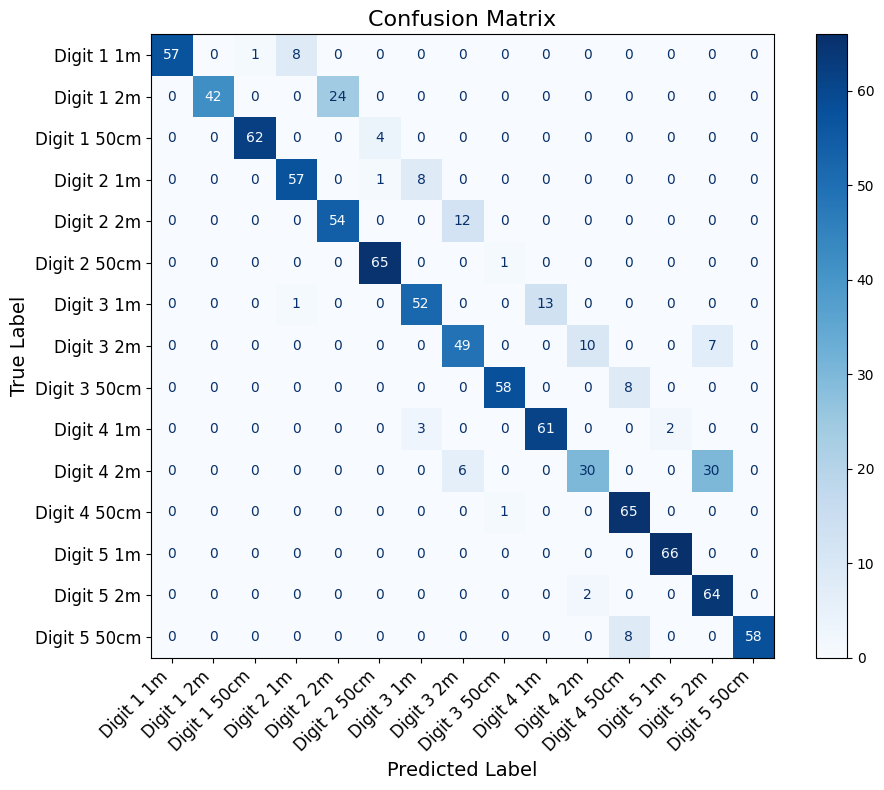
\includegraphics[width=0.7\textwidth]{Image/matrix.png}
    \caption{Confusion Matrix}
    \label{fig:confusion_matrix}
\end{figure}

\hspace{0.5cm} Confusion matrix di atas menunjukkan performa model klasifikasi untuk mendeteksi digit pada berbagai jarak (1 meter, 2 meter, dan 50 cm), di mana model berhasil mengklasifikasikan sebagian besar label dengan benar tetapi masih terdapat beberapa kesalahan prediksi yang terlihat dari nilai non-diagonal, terutama pada True Label "Digit 4 dengan jarak 2 meter", yang memiliki distribusi kesalahan tertinggi dengan salah diklasifikasikan sebagai "Digit 5 dengan jarak 2 meter" sebanyak 30 kali.
Dalam confusion matrix:

\begin{itemize}
    \begin{itemize}
        \item Warna tergelap menunjukkan nilai prediksi yang paling akurat, yaitu jumlah prediksi yang benar (true positives) untuk label tertentu. Warna ini berada pada diagonal utama matriks (misalnya, "Digit 5 pada 1 meter" dengan 66 prediksi benar).

        \item Warna yang agak terang menunjukkan adanya kesalahan klasifikasi atau prediksi yang salah (false positives atau false negatives), yang berada di luar diagonal utama. Semakin terang warnanya, semakin sedikit jumlah kesalahan untuk kombinasi label tertentu (misalnya, “Digit 2 pada 1 meter” salah diprediksi sebagai “Digit 1 pada 1 meter” sebanyak 8 kali).
    \end{itemize}
\end{itemize}

\newpage
    \item \textbf {Visualization of Training and Validation results Accuracy & Loss}
\begin{figure}[h]
    \centering
    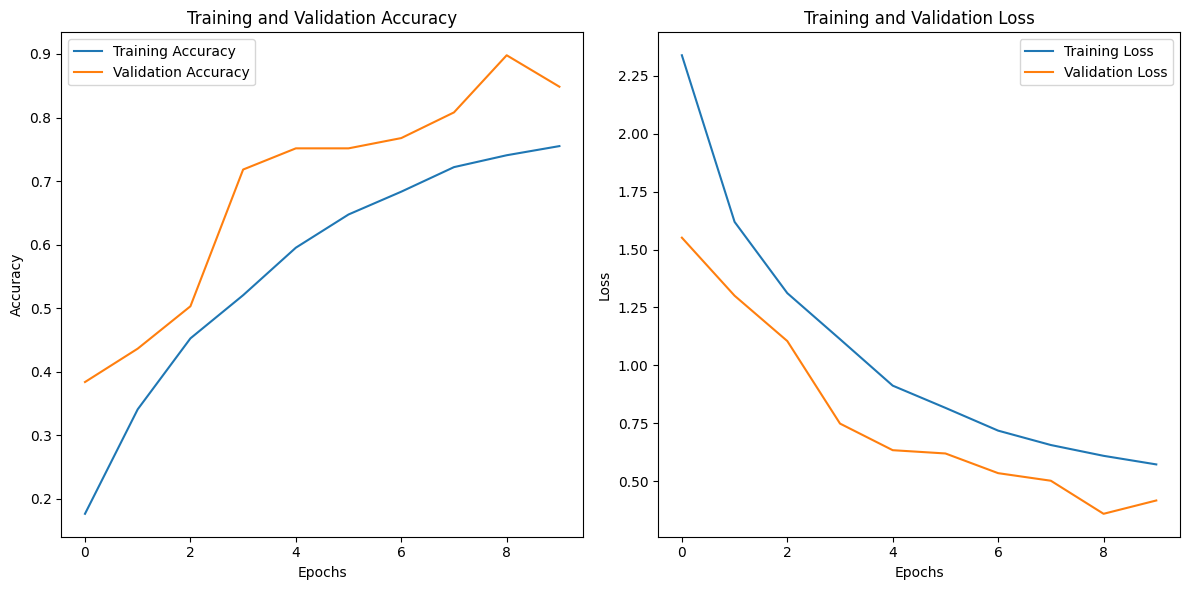
\includegraphics[width=0.7\textwidth]{Image/Grafik Train.png}
    \caption{Training and Validation Accuracy \& Loss}
    \label{fig:Training_and_Validation_Accuracy_\&_Loss}
\end{figure}

\begin{itemize}
    \begin{itemize}
        \item Training and Validation Accuracy: Akurasi meningkat secara konsisten baik untuk data pelatihan maupun validasi seiring bertambahnya epoch. Namun, pada akhir pelatihan, akurasi validasi sedikit menurun, yang dapat menjadi indikasi overfitting.

        \item Training and Validation Loss: Loss untuk data pelatihan dan validasi terus menurun selama pelatihan, menunjukkan bahwa model belajar dengan baik. Namun, pada akhir pelatihan, loss validasi tampaknya mulai sedikit meningkat, yang juga mendukung adanya kemungkinan overfitting.
    \end{itemize}
\end{itemize}

    \item \textbf{Discussion of the results, comparing them to related works}

    
    \hspace{0.5cm} Penelitian sebelumnya yang menggunakan radar berbasis Range-Doppler Map (RDM) dan pada proyek pembuatan dataset natural hand digit yang menggunakan model berbasis CNN untuk pengenalan digit tangan memiliki pendekatan berbeda dengan kelebihan dan kekurangannya masing-masing. Sistem berbasis radar dari penelitian sebelumnya mencapai akurasi tinggi sebesar 98\% untuk pengenalan gestur dinamis. Keunggulan utamanya terletak pada privasi, karena radar tidak memerlukan kamera, sehingga cocok untuk lingkungan di mana sensitivitas terhadap pelanggaran privasi menjadi prioritas. Namun, radar memiliki keterbatasan, terutama dalam mendeteksi gerakan halus atau gestur mikro. Selain itu, pengaruh lingkungan terhadap performa radar masih perlu dipahami lebih jauh.

    
    \hspace{0.5cm} Di sisi lain, proyek ini lebih berfokus pada pengenalan digit tangan statis dari 1 hingga 5 menggunakan kamera dan dataset yang variatif, yang mencakup perubahan jarak, pencahayaan, dan sudut pandang. Dengan akurasi keseluruhan sebesar 85\%, pendekatan ini menunjukkan performa yang cukup baik, terutama pada jarak dekat, di mana precision untuk beberapa digit mencapai nilai sempurna. Namun, performa pada jarak yang lebih jauh, seperti pada pengenalan digit 4 di jarak 2 meter, masih memerlukan perbaikan.

    
    \hspace{0.5cm} Keberagaman dataset yang digunakan dalam proyek ini menjadi salah satu kekuatan utama. Variasi dalam data ini memungkinkan model untuk lebih adaptif terhadap kondisi nyata, sesuatu yang kurang ditonjolkan dalam penelitian berbasis radar. Namun, pendekatan berbasis kamera juga memiliki kelemahan, terutama dalam aspek privasi dan kinerjanya di kondisi pencahayaan yang buruk.

    
    \hspace{0.5cm} Jika dibandingkan dengan karya-karya terkait lainnya, pendekatan radar seperti dalam penelitian sebelumnya sering dianggap unggul dalam privasi dan kesederhanaan sensor, tetapi terbatas dalam fleksibilitas dan resolusi detail. Sebaliknya, sistem berbasis kamera dan CNN seperti proyek ini memiliki potensi akurasi tinggi dan kemampuan untuk menangkap detail kompleks, namun dengan tantangan dalam menjaga privasi dan performa di lingkungan tertentu.

    
    \hspace{0.5cm} Dalam hal aplikasi, pendekatan radar lebih sesuai untuk sistem non-visual seperti kontrol kendaraan otonom atau perangkat rumah pintar. Sementara itu, proyek ini membuka peluang besar untuk aplikasi dalam antarmuka manusia-komputer (HCI) dan pengendalian perangkat berbasis IoT, yang membutuhkan pengenalan gestur digit tangan secara spesifik.


% 5. Conclusion

\section{\uppercase Conclusion}
\item \textbf{Recap of the objectives and how they were met}
\begin{itemize}
    \hspace{0.5cm} Proyek ini bertujuan untuk mengembangkan dataset yang mendukung pengenalan gestur tangan, khususnya hand digit dari 1 hingga 5, untuk aplikasi berbasis interaksi manusia-komputer (HCI) dan Internet of Things (IoT). Tujuan tersebut tercapai melalui pengumpulan data yang beragam dalam kondisi pencahayaan dan jarak yang berbeda, serta menggunakan teknik machine learning, khususnya Convolutional Neural Networks (CNN), untuk melatih model pengenalan gestur. Dengan menyediakan dataset yang kaya dan bervariasi, proyek ini berhasil meningkatkan akurasi dalam mengenali gestur tangan di berbagai situasi nyata.
    
    \hspace{0.5cm} Hasil dari proyek menunjukkan bahwa model yang dilatih dengan dataset ini mencapai akurasi keseluruhan sebesar 85\%. Metrik kinerja, termasuk precision dan recall, menunjukkan bahwa model dapat mengenali gestur dengan baik pada jarak yang berbeda. Misalnya, akurasi tertinggi dicapai pada digit 1 dengan jarak 50 cm, mencapai nilai 1.00 untuk precision. Selain itu, variasi dalam dataset memungkinkan model untuk lebih adaptif terhadap kondisi dunia nyata, termasuk pencahayaan rendah dan sudut pandang yang berbeda. Temuan ini menegaskan pentingnya keberagaman dalam dataset untuk meningkatkan performa model pengenalan gestur.

\end{itemize}

\item \textbf{Key insights from the results}
\begin{itemize}
        \item Digit 1 (1m, 50cm) menunjukkan precision dan F1-score yang sangat baik, mencapai 1.00 untuk precision dan 0.93-0.96 untuk F1-score, menunjukkan pengenalan yang sangat baik.

        \item Digit 2 (2m) memiliki precision yang lebih rendah (0.69) tetapi recall yang lebih baik (0.82), yang menunjukkan bahwa meskipun tidak terlalu presisi, model dapat mengenali banyak gambar dengan benar.

        \item Digit 4 (2m) menunjukkan nilai precision dan recall yang lebih rendah, terutama pada precision (0.71) dan recall (0.45), yang menunjukkan tantangan dalam mengenali gestur ini pada jarak 2m.

        \item Digit 5 (50cm) memiliki precision 1.00 dan F1-score yang tinggi, menunjukkan kinerja model yang sangat baik dalam mengenali gestur ini pada jarak dekat (50cm).

        \item Secara keseluruhan, Digit 1, 2, 3, dan 5 memiliki kinerja yang sangat baik, tetapi Digit 4 pada jarak 2m perlu ditingkatkan.
\end{itemize}

\item \textbf{Future work and recommendations}
\begin{itemize}

    \hspace{0.5cm} Ke depan, disarankan agar penelitian ini diperluas dengan menambahkan lebih banyak variasi dalam dataset, terutama menambah data untuk kelas-kelas yang memiliki akurasi rendah, seperti Digit 4 (2m), untuk meningkatkan keakuratan prediksi. Selain itu, melakukan augmentasi lebih lanjut pada kelas-kelas dengan F1-score rendah untuk memperbaiki kemampuan model dalam mengenali variasi gestur pada jarak tertentu. Penelitian lebih lanjut juga dapat mencoba model yang lebih kompleks seperti ResNet atau menggunakan transfer learning untuk meningkatkan kinerja, terutama pada kelas yang sulit dikenali. Dengan terus mengembangkan dan memperbaiki dataset serta metodologi pelatihan, potensi aplikasi teknologi pengenalan gestur tangan dapat dimaksimalkan di berbagai bidang.

\end{itemize}





\begin{thebibliography}{999}

\bibitem{Bender2012}
Bender, A., \& Beller, S. Nature and culture of finger counting: Diversity and representational effects of an embodied cognitive tool. {\em Cognition} {\bf 124}(2), 156--182. DOI: \url{https://doi.org/10.1016/j.cognition.2012.05.005}.

\bibitem{Ahlawat2020}
Ahlawat, S., \& Choudhary, A. Hybrid CNN-SVM Classifier for Handwritten Digit Recognition. {\em Procedia Computer Science} {\bf 167}, 2554--2560. DOI: \url{https://doi.org/10.1016/j.procs.2020.03.309}.

\bibitem{Jhaung2022}
Jhaung, Y. C., Lin, Y. M., Zha, C., Leu, J. S., \& Köppen, M. Implementing a Hand Gesture Recognition System Based on Range-Doppler Map. {\em Sensors} {\bf 22}(11). DOI: \url{https://doi.org/10.3390/s22114260}.

\end{thebibliography}

\end{document}
